\documentclass[12pt]{article}
\usepackage[margin=1in]{geometry}
\usepackage{amsmath}
\usepackage{siunitx}
\usepackage{graphicx}
\usepackage{subcaption}

\begin{document}

\title{DD2424 Deep Learning in Data Science Assignment 1 Ex. 1}
\author{Lin Chun Hung, chlin3@kth.se}

\maketitle

In this exercise, a python version of multi-linear classifier was implemented.
The function to compute the gradient with analytical method was competed.

Unit tests for the function computing the gradient were written. In those unit tests,
I used \texttt{numpy.testing.assert\_allclose} to check if all the elements of two pairs of gradients,
\texttt{gradW} and \texttt{gradb}, computed from the analytical method and the numerical methods are closed.
In the assertion, the following equation is element-wise true, otherwise the unit test will fail.

\begin{equation*}
    % absolute(a - b) <= (atol + rtol * absolute(b))
    |a - b| \leq (\texttt{atol} + \texttt{rtol} * |b|)
\end{equation*}
where \texttt{atol} and \texttt{rtol} are the tolerance parameters.

Since the forward difference method is less accurate than the central difference method,
the tolerance parameters are different when comparing them to analytical method.
I set \texttt{atol} as \num{1e-7} and \texttt{rtol} as \num{1e-06} for the
forward difference method and set \texttt{atol} as \num{1e-9} and \texttt{rtol} as \num{1e-07}
for the central difference method.


\begin{figure}
    \centering
    \begin{subfigure}[b]{0.475\textwidth}
        \centering
        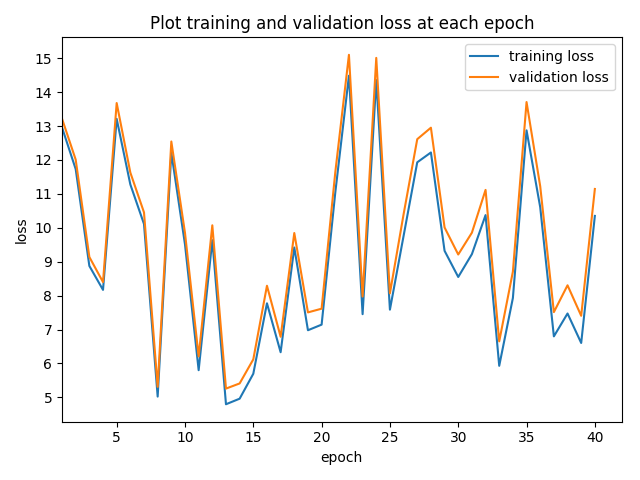
\includegraphics[width=\textwidth]{loss_case1.png}
        \caption[]%
        {{\small Network 1}}
        \label{fig:mean and std of net14}
    \end{subfigure}
    \hfill
    \begin{subfigure}[b]{0.475\textwidth}
        \centering
        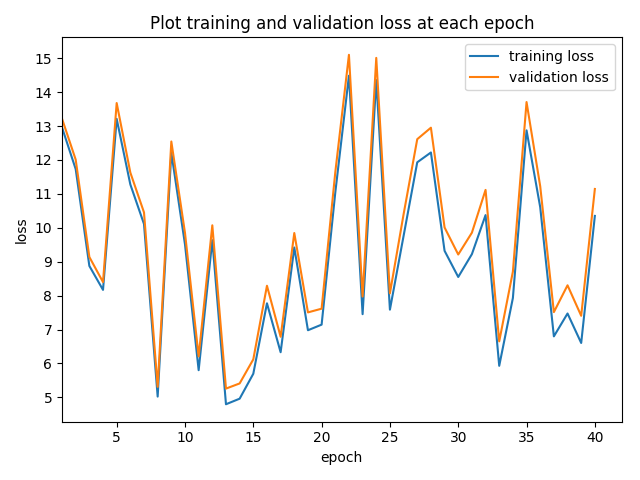
\includegraphics[width=\textwidth]{loss_case1.png}
        \caption[]%
        {{\small Network 2}}
        \label{fig:mean and std of net24}
    \end{subfigure}
    \vskip\baselineskip
    \begin{subfigure}[b]{0.475\textwidth}
        \centering
        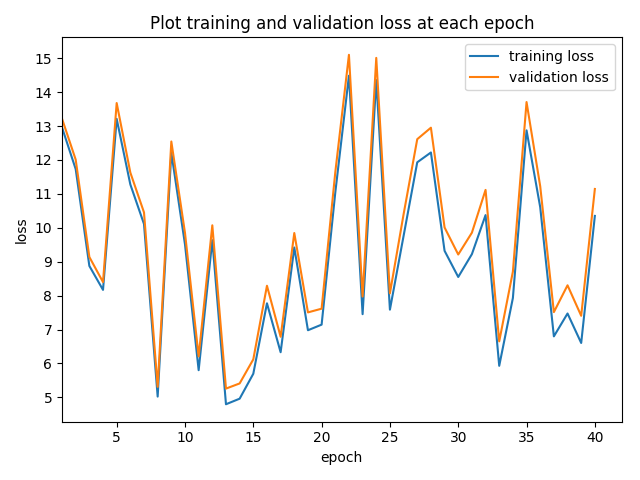
\includegraphics[width=\textwidth]{loss_case1.png}
        \caption[]%
        {{\small Network 3}}
        \label{fig:mean and std of net34}
    \end{subfigure}
    \quad
    \begin{subfigure}[b]{0.475\textwidth}
        \centering
        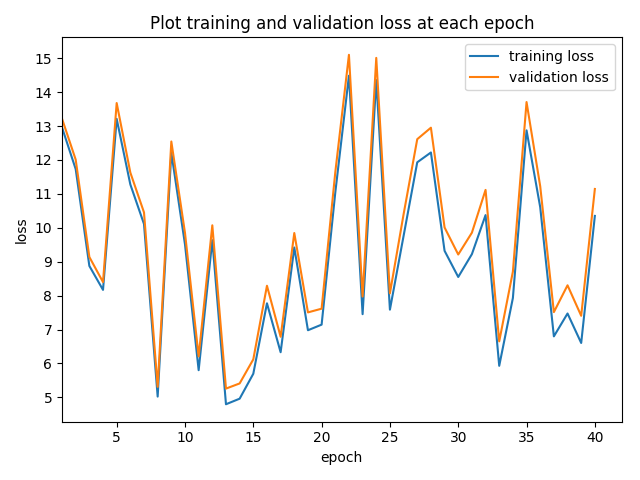
\includegraphics[width=\textwidth]{loss_case1.png}
        \caption[]%
        {{\small Network 4}}
        \label{fig:mean and std of net44}
    \end{subfigure}
    \caption[ The average and standard deviation of critical parameters ]
    {\small The average and standard deviation of critical parameters: Region R4}
    \label{fig:mean and std of nets}
\end{figure}
\end{document}
